\documentclass[tikz]{standalone}

\usetikzlibrary{arrows, shapes, positioning}

\begin{document}
    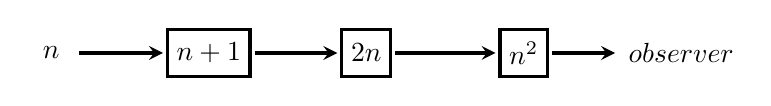
\begin{tikzpicture}[scale=4, >=stealth, node distance=2cm, shorten >=1pt, shorten <=1pt, minimum size=0.6cm, very thick]
        \node[] (data) {$n$};
        \node[rectangle, draw, right of=data] (incrementer) {$n+1$};
        \node[rectangle, draw, right of=incrementer] (doubler) {$2n$};
        \node[rectangle, draw, right of=doubler] (squarer) {$n^2$};
        \node[right of=squarer] (observer) {$observer$};

        \draw[->] (data) -- (incrementer);
        \draw[->] (incrementer) -- (doubler);
        \draw[->] (doubler) -- (squarer);
        \draw[->] (squarer) -- (observer);
    \end{tikzpicture}
\end{document}
